\documentclass[a4paper, twocolumn, 11pt, twoside]{article}

\usepackage[brazil]{babel}
\usepackage{linguamatica}
\usepackage{expex}

\usepackage{linguex}
\usepackage[utf8]{inputenc} % To handle special characters
\usepackage{amssymb} % For symbols like ? in glosses
%\usepackage{microtype}

\usepackage{mathtools, amsmath, float} 
\usepackage{MnSymbol} %M: para a Defeasible Implication

\usepackage[T1]{fontenc}
\usepackage{xcolor}   % For color
\usepackage{graphicx} % For handling images (optional)
\usepackage{fancyhdr} % For custom headers/footers (optional)

\definecolor{ForestGreen}{RGB}{34,139,34}
\definecolor{Maroon}{RGB}{128,0,0}

\definecolor{lightgray}{RGB}{224, 224, 224}
\definecolor{mblue}{RGB}{0, 127, 204}
\definecolor{lightyellow}{RGB}{255, 247, 209}
\definecolor{lightblue}{RGB}{204, 230, 255} % 

%% Please use UTF8 in your document

%% Set the bibliography style.
%% Styles provided for Spanish (Castilian), Catalan and Portuguese.
%% Other languages will be created on a required basis.

\bibliographystyle{sp_por}   % This for Portuguese
% \bibliographystyle{sp_esp} % This for Castilian
% \bibliographystyle{sp_cat} % This for Catalan


%% You can leave this unchanged. It will be updated by the editors when your paper gets published.
\submitted{15 de \OCT{} 2024}
\accepted{3 de \DEC{} 2024}


%% Add your title in the main language used in the article
\title{Desafios na Tradução de Informação Espacial do Inglês para o Português}

%% Currenty the title in English is also mandatory
\titleEN{Challenges in Translating Spatial Information from English to Portuguese}


%% Add authors here. Three lines for each author.
%% First line with author name, second with the affiliation and third with e-mail
%% In cases where a second line is needed for the affiliation, use the command \nl to separate them. 
\author{
  Rafael Fernandes
  \instituto{Universidade de São Paulo}
  \email{rafael.macario@usp.br} 
  \and 
  Rodrigo Souza
 \instituto{Universidade de São Paulo}
  \email{rodrigo.aparecido.souza@usp.br}
  \and
  Marcos Lopes
  \instituto{Universidade de São Paulo}
  \email{marcoslopes@usp.br}
  \and
%%  Paulo Santos
%%  \instituto{Flinders University}
%%  \email{paulo.santos@flinder.edu.au}
%%%%  \and
%%  Thomas Finbow
%%  \instituto{Universidade de São Paulo}
%%  \email{thomas.finbow@usp.br}
}


\begin{document}
\maketitle

%% Add the abstract in the main language for the article. If possible, doesn't add any citations here.
\begin{resumo}
Os sistemas de Tradução Automática Neural (TAN), atualmente a abordagem mais utilizada na Tradução Automática, ainda enfrentam desafios ao lidar com a tradução da linguagem espacial. Neste estudo, utilizamos o Raciocínio Espacial Qualitativo (REQ) para representar informações espaciais nas traduções automáticas do inglês para o português. Traduzimos 145 frases dos corpora CAM e COCA, utilizando Google Translate e DeepL, e identificamos as causas das traduções não naturais. Com o uso do REQ, mapeamos logicamente as diferenças de significado. Nossos resultados indicam que, apesar do bom desempenho geral, os motores TAN apresentam dificuldades com significados espaciais específicos, resultando em $10,6\%$ de erros semânticos e $12,0\%$ de erros de projeção sintática. Este trabalho explora os desafios práticos e teóricos da tradução automática.
\end{resumo}

%% Add keywords in the article main language, in lowercase
\palavraschave{Tradução Automática Neural; Tradução Automática Inglês-Português; Raciocínio Espacial Qualitativo; Google Translate; DeepL.}


%% Add the abstract in English
\begin{abstract}
\end{abstract}

%% add the keywords in English
\keywords{Open-source LLMs, Neural Machine Translation, Spatial Semantics, Polysemy, Language Typology}


\section{Introdução}

A Tradução Automática Neural (TAN) tornou-se o paradigma dominante na área de Tradução Automática (TA), tanto em estudos acadêmicos quanto em aplicações práticas~\citep{dabre2020survey}. Esse avanço se deve, em grande parte, à capacidade aprimorada dos modelos de aprendizado profundo de captar dependências longas nas frases~\citep{vaswani2017attention, yang2020survey}.

No entanto, apesar de serem bastante eficientes, alguns tradutores automáticos ainda enfrentam desafios ao lidar com as sutilezas da linguagem espacial, como a polissemia das preposições e a projeção idiossincrática da maneira do movimento em inglês diretamente em verbos no português~\citep{McCleary-Viotti-2004}. Um exemplo disso pode ser observado no Exemplo (1), retirado do Cambridge Online Dictionary (CAM), onde a tradução do inglês (EN) para o português (PT) foi realizada com o Google Translate (GT) e o DeepL (DL).


\subsection{Desafios na Tradução da Espacialidade}

A formatação ao longo do documento é a normal em documentos \LaTeX, sem grandes alterações. No entanto,
algumas sugestões:
\begin{itemize}
\item Para dar \emph{ênfase} use sempre que possível o comando \verb.\emph.;
\item Para citar poderá usar o comando \verb.\citep. que cria referências entre
  parêntesis~\citep{latex}. Para citar um \citet{autor}, use o comando \verb.\citet.;
\item Citações seguidas devem reaproveitar o comando de citação. Caso necessite de indicar a página
  a que se refere a citação, use \citep[p.~40]{latex}.
\item Ao criar entradas bibliográficas assegure-se da correção do seu
  conteúdo. Não abrevie nomes de autores. Não coloque os nomes dos
  editores de livros de atas. Não se esqueça dos números das páginas
  do documento.
\item Sempre que usar endereços web e outros tipos de URI, coloque-os com o comando \verb.\url. e,
  sempre que possível, em nota de fim de página.\footnote{Assim. \url{http://www.linguamatica.com}}
\item Nas notas de fim de página que sejam anexadas a palavras seguidas de pontuação, devem ser colocadas
  após a pontuação, como exemplificado no item anterior.
\item Tenha em atenção a diferença entre -, -- e ---. O primeiro será usado entre palavras, como em
  curto-circuito, o segundo em intervalos, como 10--20 ou PT--EN e o terceiro --- este --- para
  introduzir pequenos comentários.
\item As figuras devem ser legendadas e a legenda deve terminar com um sinal de pontuação.
\item As referências a figuras, tabelas ou secções devem ser criadas usando as ferramentas do \LaTeX{}.
\item Sempre que possivel garanta a qualidade das imagens importadas, usando PDF ou PNG.
\item Ao criar tabelas (Tabela~\ref{tab:1}) tente diminuir a quantidade de traços usada. Grande parte das
  tabelas são legíveis apenas com um par de linhas como demonstrado.
\end{itemize}

\begin{table}[htb]
  \centering
  \begin{tabular}{lrr}
    \toprule
    & \textbf{Homens} & \textbf{Mulheres} \\
    \midrule
    Crianças & 10~032 & 32~341 \\
    Adultos & 23~431 & 9~443 \\
    \bottomrule
  \end{tabular}
  \caption{Exemplo de tabela com poucos traços.}
  \label{tab:1}
\end{table}

\section{Metodologia}
Nesta seção, apresentamos as etapas metodológicas do nosso trabalho, composta pela coleta dos dados, pela classificação das preposições, pelo processo de tradução, pelas formalizações das informações espaciais e pela categorização das traduções. 

\subsection{Coleta dos Dados}

\subsection{Classificação das Preposições}

\subsection{Tradução das Sentenças}

%\subsection{Formalização das Informações Espaciais}

\subsection{Formalização das Sentenças}

A partir do trabalho de~\citet{spranger2016robust}, definimos cada intervalo de tempo $t$ como um conjunto de pontos e utilizamos o predicado \textit{occurs\_in($\theta$, $t$)} para denotar que um evento $\theta$ ocorre durante um intervalo de tempo $t$.
Com base em~\citet{freksa2016neighborhood}, definimos os eventos $\theta$ por meio do cojunto de treze relações qualitativas espaço-temporais apresentadas na Figura~\ref{fig:13_relations}.

\begin{figure}[ht]
	\centering
	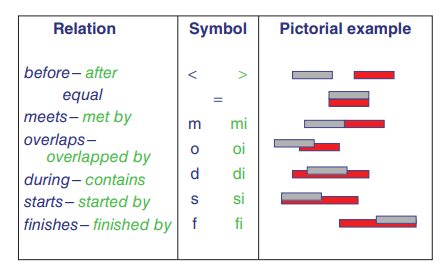
\includegraphics[width=\columnwidth]{Figures/13_concep_neigb_relat.png}
	\caption{Treze relações qualitativas entre dois objectos lineares estendidos sobre uma reta orientada~\citep{freksa2016neighborhood}.}
	\label{fig:13_relations}
\end{figure}

A Figura~\ref{fig:13_relations} apresenta  as treze relações conjuntamente exaustivas e em pares disjuntivos baseadas no Cálculo de Intervalos de Allen~\citep{allen1983maintaining}.
Essas relações podem ser descritas pelo seguinte cojunto: \{\textit{before, after, equal, meets, met by, overlaps, overlapped by, during, contains, starts, started by, finishes, finished by}\}. 
Com esse cojunto de relações, podemos representar transições relacionadas ao movimento de objetos que fazem parte de um evento.

Por \textit{default}, assumimos um espaço 3D para todos os objetos em nossas representações de movimento nas cenas. Para representar as informações espaciais em sentenças como as do Exemplo (1), em que a preposição ``across'' denota
o movimento de atravessar uma superfície, definimos uma função \textit{surface(r)}. Essa função mapeia relações como
\textit{during} ou \textit{contains}, projetando um objeto em uma superfície 2D.

Para modelar relações mereotopológicas, nos baseamos no RCC-8~\citep{randell1992spatial}: \{\textit{dc, ec, po, eq, tpp, ntpp, tpp}${^{-1}}$, \textit{ntpp}${^{-1}}$\}.
Para formalizar uma sentença como a gerada pela tradução do GT no Example~\ref{example:across2}, nós definimos uma Região de Referência (\textit{RR}), que é uma parte de 
uma região \textit{R}, ou Fundo, localizada fora da região onde a ação executada pelo objeto \textit{F}, a Figura, 
acontece. A Região de Referência é separada do restante de \textit{R} por uma linha transversal (chamada por nós de \textit{meridiano}) 
que liga com \textit{R} em dois pontos distantes (não consecutivos) e não toca $F: R_{op} = ntpp(F, R)$.

De modo a representar a relação entre o predicado \textit{occurs\_in($\theta$, $t$)} e as relações qualitativas 
apresentadas na Figura~\ref{fig:13_relations}, nós utilizamos o conectivo $\leftlsquigarrow$, que denota uma implicação
revogável, isto é, uma forma de raciocíno que é racionalmente convincente, mas carece de validade dedutiva. 
Nesse contexto, as premissas do argumento oferecem suporte racional para a conclusão, mas há a possibilidade 
de as premissas serem verdadeiras e a ser falsa. Em resumo, a conexão entre as premissas e a conclusão são provisórias
e podem ser anuladas por informações suplementares.

\subsection{Categorização das Traduções}
%\subsection{title}

\section{Resultados e Discussão}


\begin{table}[!htb]
  \centering
  \scalebox{0.8}{
  \begin{tabular}{| l |p{.3\textwidth}|}%{|l|l|}
  \hline
  \textbf{Original text:} He swam \underline{across} the river. 
  \\\hline\hline
  \begin{tabular}[c]{@{}l@{}}  
  $\forall t$ $ \in \{t_1, t_2, t_3\}, t_1 < t_2 < t_3$\\ 
  $occurs\_in(moves\_across(he, river), t)$ $\leftlsquigarrow$\\
  $river' = surface(river)$ $\wedge$\\
  $starts(he, river', t_1)$ $\wedge$\\ 
  $during(he, river', t_2)$ $\wedge$\\ 
  $finishes(he, river', t_3)$\\
  %$continuous(t_1, t_2, t_3)$\\
  
  \end{tabular}\\\hline\hline
  \textbf{GT:} Ele nadou \underline{do outro lado} do rio. 
  \\\hline\hline
  \begin{tabular}[c]{@{}l@{}}  
  
  $\forall t$ $\in \{t_1, t_2, t_3\}, t_1 < t_2 < t_3$\\
  $occurs\_in(moves\_on\_opposite\_side(he, river_{op}), t)$ $\leftlsquigarrow$\\
  $river' = surface(river_{op})$ $\wedge$\\
  $starts(he, river', t_1)$ $\wedge$\\
  $during(he, river', t_2)$ $\wedge$\\ 
  $finishes(he, river', t_3)$\\
  \end{tabular}\\\hline\hline
  
  \textbf{DL:} Ele \underline{atravessou} o rio a nado.
  \\\hline\hline
  \begin{tabular}[c]{@{}l@{}} 
  $\forall t$ $ \in \{t_1, t_2, t_3\}, t_1 < t_2 < t_3$\\ 
  $occurs\_in(moves\_across(he, river_{op}), t)$ $\leftlsquigarrow$\\
  $river' = surface(river_{op})$ $\wedge$\\
  $starts(he, river', t_1)$ $\wedge$\\ 
  $during(he, river', t_2)$ $\wedge$\\ 
  $finishes(he, river', t_3)$\\
  % $continuous(t_1, t_2, t_3)$\\
  \end{tabular}\\\hline
  
  \end{tabular}}
  \caption{Formalizations for sentences in Example~\ref{example:across2}.}
  \label{table:FormAcross}
  \end{table}


  % Through
\begin{table}[!htb]
  \centering
  \scalebox{0.7}{
  \begin{tabular}{| l |p{.3\textwidth}|}%{|l|l|}
  \hline
  \textbf{Original text:} He struggled \underline{through} the crowd till he\\ reached the front.
  \\\hline\hline
  \begin{tabular}[c]{@{}l@{}}  
  $\forall t$ $\in \{t_1, t_2, t_3\}, t_1 < t_2 < t_3$\\ $occurs\_in(arduously(moves\_through(he, crowd), t))$ $\leftlsquigarrow$\\ 
  $starts(he, crowd, t_1)$ $\wedge$\\  
  $during(he, crowd, t_2)$ $\wedge$\\ 
  $finishes(he, crowd, t_3)$ \\
  \end{tabular}\\\hline\hline
  
  \textbf{GT:} Ele lutou \underline{no meio} da multidão até chegar à frente. 
  \\\hline\hline
  \begin{tabular}[c]{@{}l@{}} 
  $\forall t$ $\in \{t_1, t_2, t_3\}, t_1 < t_2 < t_3$\\
  $occurs\_in(fights(he, crowd)$ $\wedge$ $moves\_to(he, crowd), t)$ $\leftlsquigarrow$\\
  $starts(he, crowd, t_1)$ $\wedge$\\  
  $during(he, crowd, t_2)$ $\wedge$\\ 
  $finishes(he, crowd, t_3)$\\ 
  \end{tabular}\\\hline\hline
  
  \textbf{DL:} Ele se debateu \underline{entre} a multidão até chegar à frente.
  \\\hline\hline
  \begin{tabular}[c]{@{}l@{}} 
  $\forall t$ $\in \{t_1, t_2, t_3\}, t_1 < t_2 < t_3$\\
  $occurs\_in(flounder(he, crowd)$ $\wedge$ $moves\_to(he, crowd), t)$ $\leftlsquigarrow$\\
  $starts(he, crowd, t_1)$ $\wedge$\\  
  $during(he, crowd, t_2)$ $\wedge$\\ 
  $finishes(he, crowd, t_3)$\\  
  \end{tabular}\\\hline
  \end{tabular}}
  \caption{Formalizations for sentences in Example~\ref{example:through1}.}
  \label{table:FormThrough}
  \end{table}



  
  
 
\section{Conclusão}

\section*{Agradecimentos}

Os agradecimentos devem ser colocados sempre numa secção final, sem número, tal como
neste exemplo. Sempre que o autor assim o entender, deverá agradecer aos revisores.


\bibliography{references.bib}


\end{document}
